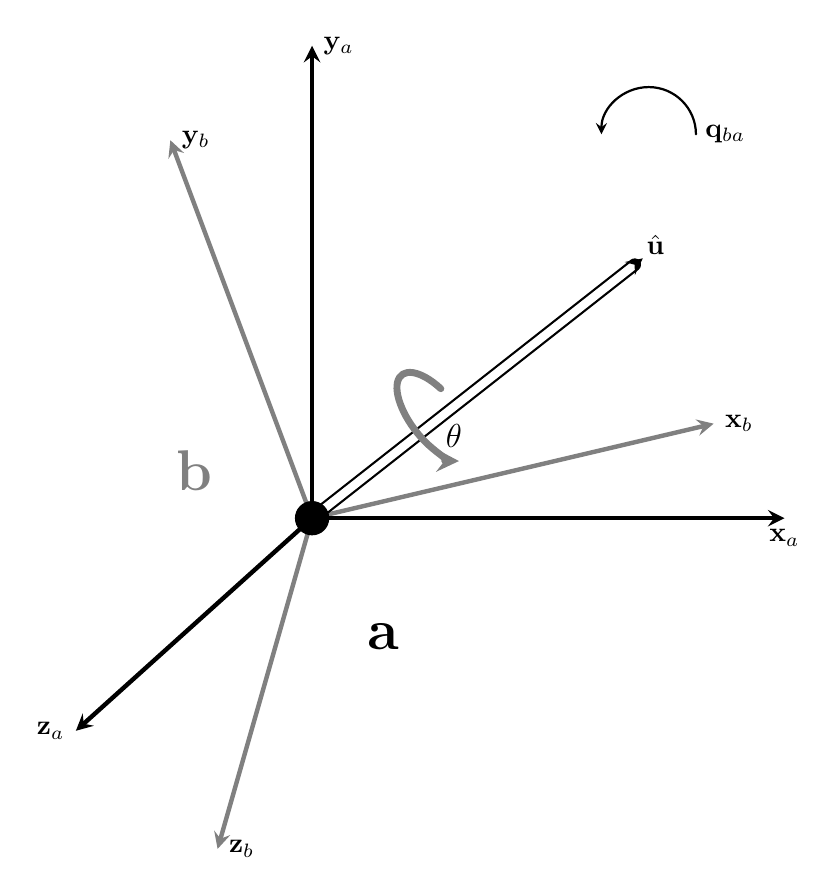
\begin{tikzpicture}[>=stealth, scale=1.5, line cap=round, line join=round]

    % ------------------------------------------------------------------
    % 1. Frame b (Rotated Frame)
    % Drawn first so it sits slightly behind the origin and Frame a
    % ------------------------------------------------------------------
    \draw[->, ultra thick, gray] (0,0) -- (3.4, 0.8) 
        node[right, text=black] {$\mathbf{x}_b$};
    \draw[->, ultra thick, gray] (0,0) -- (-1.2, 3.2) 
        node[right, text=black] {$\mathbf{y}_b$};
    \draw[->, ultra thick, gray] (0,0) -- (-0.8, -2.8) 
        node[right, text=black] {$\mathbf{z}_b$};

    % ------------------------------------------------------------------
    % 2. Frame a (Initial Frame)
    % ------------------------------------------------------------------
    \draw[->, ultra thick, black] (0,0) -- (4,0) 
        node[below] {$\mathbf{x}_a$};
    \draw[->, ultra thick, black] (0,0) -- (0,4) 
        node[right] {$\mathbf{y}_a$};
    \draw[->, ultra thick, black] (0,0) -- (-2,-1.8) 
        node[left] {$\mathbf{z}_a$};

    % ------------------------------------------------------------------
    % 3. Unit Rotation Axis (u)
    % Uses a double line to mimic the thick outline arrow in the image
    % ------------------------------------------------------------------
    \draw[->, double=white, double distance=3pt, thick, black] 
        (0,0) -- (2.8, 2.2) 
        node[above right, text=black, font=\bfseries, inner sep=1pt] {$\hat{\mathbf{u}}$};

    % ------------------------------------------------------------------
    % 4. Origin Marker (Drawn last to cover line intersections cleanly)
    % ------------------------------------------------------------------
    \filldraw[black] (0,0) circle (4pt);

    % ------------------------------------------------------------------
    % 5. Frame Identifiers (a and b)
    % ------------------------------------------------------------------
    \node[font=\huge\bfseries, black] at (0.6, -1.0) {a};
    \node[font=\huge\bfseries, gray] at (-1.0, 0.4) {b};

   % ------------------------------------------------------------------
    % 6. Theta rotation about the axis u (perpendicular perspective)
    % ------------------------------------------------------------------
    % Center of the arc positioned along u at (1.26, 0.99)
    \begin{scope}[shift={(1.26, 0.99)}, rotate=128]
        \draw[->, line width=2.5pt, gray]
            (160:-.2cm and 0.2cm) arc[start angle=-70, end angle=160, x radius=0.45cm, y radius=0.2cm];
    \end{scope}
    
    % Label offset slightly from the arc center
    \node[font=\large] at (1.2, .7) {$\theta$};

    % ------------------------------------------------------------------
    % 7. Quaternion rotation symbol (q_{b,a})
    % ------------------------------------------------------------------
    \draw[->, thick, black] 
        (3.25, 3.25) arc[start angle=0, end angle=180, radius=0.4] 
        node[pos=0, right, inner sep=3pt] {$\mathbf{q}_{ba}$};

\end{tikzpicture}